\section{Introduction}
In 1978, Thomas C. Schelling developed his tipping model by placing pennies and dimes on a chess board and moved them according to various rules. 
By viewing the pennies and dimes as two types of people, the rule of moving as a preference for the individuals, and the chess board as a city, he soon discovered that segregation takes place on the board, even when the preference of an individual is very subtle.\\
\\
Based on this idea, we created a basic model which consists of an $8\times8$ board with $40$ individuals that are divided evenly into two types. 
The individuals are moved according to their 'Happiness' in the current place. 
For the basic model, an individual is considered happy if $\frac{1}{3}$ of his/her second order neighbours (a person has at most $8$ neighbours) shares his type. 
Otherwise, an individual is considered unhappy and will move to the nearest place where  his/her happiness is strictly higher. This will be referred to as the 'Happiness Rule'.\\
\\ 
An example of the basic model is given below. It is clear that not every individual in figure \ref{fig:ebmb} is happy. After segregation the individuals have relocated themselves as in figure \ref{fig:ebme}, there every individual is happy.

\begin{figure}[H]
	\centering
    \begin{subfigure}{0.45\textwidth}
        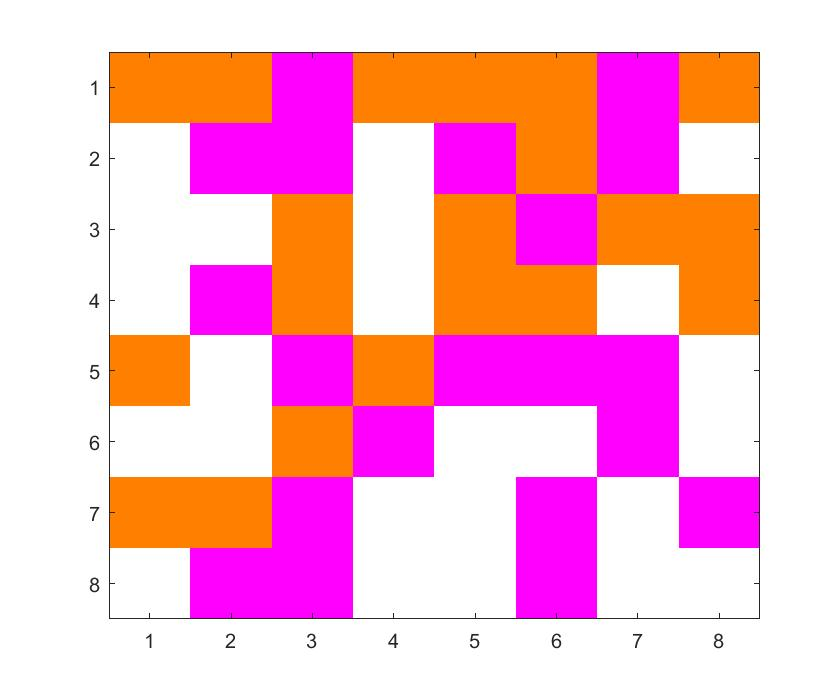
\includegraphics[width=\textwidth]{vb1beginbord.jpg}
        \caption{Situation before segragation}
        \label{fig:ebmb}
    \end{subfigure}\hspace{0cm}
    ~ 
    \begin{subfigure}{0.45\textwidth}
        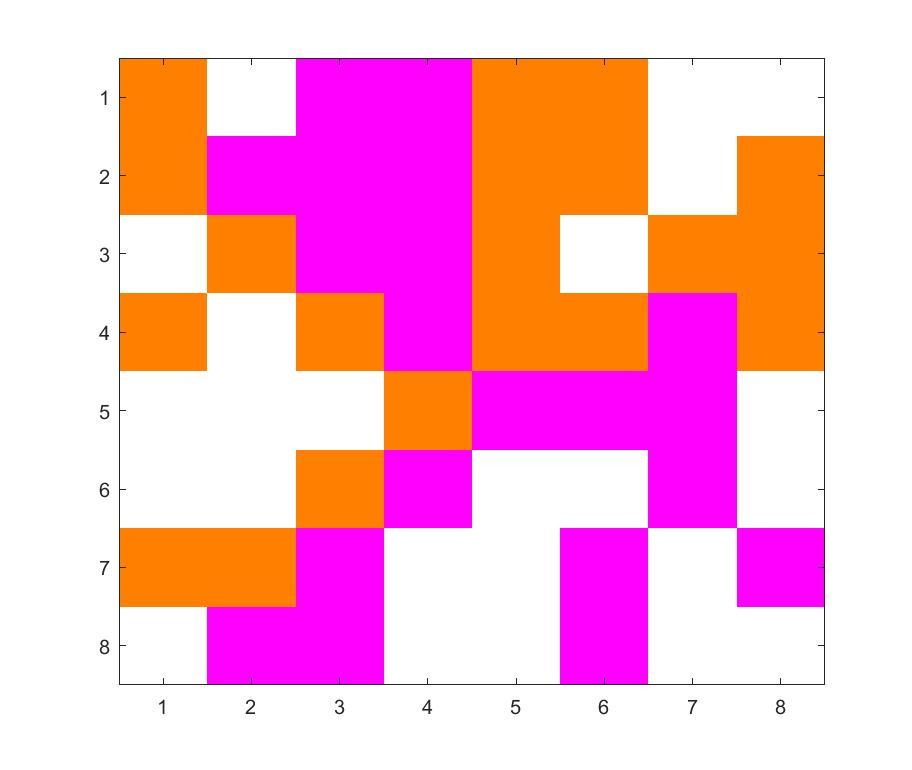
\includegraphics[width=\textwidth]{vb1eindbord.jpg}
        \caption{Situation after segregation}
        \label{fig:ebme}
    \end{subfigure}
    ~ 
    \caption{An example of segregation in our basic model: type 1 is orange and type 2 is pink}
    \label{fig:example basic model}
\end{figure}

After that, we extended the basic model by changing the parameters such as the size of the population, the boardsize and the number of types. 
We also included an option for random displacement: an individual which is not happy will be moved to a empty location chosen at random (with homogenous probability).\\
\\
For both the basic and the extended model, we ran $500$ simulations multiple times and investigated to what extent certain parameters affected the segregation pattern. 
In order to formulate our research goals precisely, the following definitions are introduced:\\
1. \textbf{Generation}: 
A population is said to have entered the next generation if the happiness of every individual has been checked once. \\
2. \textbf{Equilibrium after \(g\) generations}: 
The population is said to have reached an equilibrium after \(g\) generations if no individual has moved during the \(g+1\)-th generation.\\
3. \textbf{Homogeneity}:
A person is said to live homogenous if all of his/her neighbours share his type.\\
4. \textbf{Segregation time at $n\%$}: 
The segregation time at $n\%$ is defined as the number of generations after which $n\%$ of the population is homogenous.\\
\\
For the following sections, when it is not specified whether some parameters has been changed, one may always assume that these parameters are of the standard models.
\newpage
For the analysis, we focused on the following main questions:
\begin{enumerate}
	\item 	Does the population always reach an equilibrium? 
	How many generations on average does it take to reach an equilibrium? 
	How does the Happiness Rule affect the number of generations til equilibrium? 
	What's the probability distribution of the number of generations to reach an equilibrium?

	\item What is the average segregation time at \(60\%\), \(80\%\) and \(100\%\). 
	How is this segreggation time distributed with Happiness Rule \(1\) and how does the Happiness Rule affect the average segregation time?
	
	\item If an individual is able to switch to another type with a probability that depends on the type of it's neighbours,
	How does this affect the average number of generations(until equilibrium) and it's distribution and the other questions posed above?
\end{enumerate}

